\chapter{آموزش شبکه، Embedding بافتی و تبدیل نویسه به واج}

این فصل سه بخش دارد: مرور آموزش شبکه (لایهٔ خروجی، آموزش در برابر استنتاج، بیش‌برازش)؛ \eng{Embedding}های بافتی، \eng{BERT}، قیاس برداری و \term{کاوش}{Probing}؛ و بازگشت به \eng{TTS} برای یافتن تلفظ درست هر واژه (هم‌نویسه‌ها و \eng{G2P}). مفاهیم پایهٔ آموزش (انتشار رو‌به‌جلو، خطا، پس‌انتشار، $w_{\text{new}}=w_{\text{old}}-\eta\,\partial E/\partial w$) در فصل قبل آمده‌اند.

\section{مرور فرایند آموزش شبکهٔ عصبی}

\subsection{طراحی لایهٔ خروجی بر اساس نوع مسئله}
نکتهٔ مورد تأکید استاد: \emph{خروجی شبکه باید با \eng{Task} هم‌خوان طراحی شود.}

\begin{table}[htbp]
\centering
\small
\begin{tabular}{p{2.6cm}p{3.4cm}p{3.3cm}p{3.5cm}}
\toprule
\textbf{نوع مسئله} & \textbf{لایهٔ خروجی} & \textbf{تابع خطا} & \textbf{مثال}\\
\midrule
\eng{Regression} & یک خروجی خطی (مقدار پیوسته) & \eng{MSE} & پیش‌بینی فرکانس پایه\\
\eng{Binary Classification} & یک خروجی \eng{Sigmoid} و آستانه‌گذاری & \eng{Binary Cross-Entropy} & واکدار/بی‌واک، گفتار/سکوت\\
\eng{Multi-class Classification} & \eng{Softmax} روی \eng{K} کلاس & \eng{Cross-Entropy} & نوع احساس صدا، تلفظ درست یک واژه\\
\bottomrule
\end{tabular}
\caption{ارتباط نوع مسئله با لایهٔ خروجی و تابع خطا.}
\end{table}

\begin{itemize}
  \item \textbf{رگرسیون:} اگر شبکه بردار $X\in\mathbb{R}^{1\times 768}$ ساخته باشد، یک لایهٔ خطی $W\in\mathbb{R}^{768\times1}$ می‌دهد $Y=XW+b$. اگر مسئله پیچیده‌تر باشد، \eng{Linear $\rightarrow$ Activation $\rightarrow$ Linear} (یک \eng{MLP}) به‌کار می‌رود؛ استاد تأکید کرد پیچیده‌ترکردن باید بر اساس عملکرد باشد.
  \item \textbf{دودویی:} خروجی یک \term{لاجیت}{Logit} است که از سیگموید $\sigma(x)=1/(1+e^{-x})\in(0,1)$ می‌گذرد؛ مثلاً $0.8$ یعنی احتمال کلاس مثبت ۸۰ درصد، و با یک آستانه (\eng{Threshold}) کلاس نهایی تعیین می‌شود.
  \item \textbf{چندکلاسه:} \eng{Softmax} لاجیت‌ها را به توزیع احتمال با مجموع ۱ تبدیل می‌کند:
\end{itemize}
\[
P(y=i)=\frac{e^{z_i}}{\sum_{j=1}^{K}e^{z_j}},\qquad \sum_{i=1}^{K}P(y=i)=1 .
\]
در پیش‌بینی توکن بعدی با واژگان $V$ توکن، بردار $1\times768$ در ماتریس $768\times V$ ضرب می‌شود و بردار لاجیت $1\times V$ حاصل می‌شود.

\subsection{تابع خطا و مثال پیش‌بینی توکن بعدی}
برای برچسب \eng{One-Hot}، \eng{Cross-Entropy} ساده می‌شود به
$L=-\sum_k y_k\log \hat y_k = -\log \hat y_{c}$
که در آن $c$ کلاس درست است؛ یعنی فقط احتمالی که مدل به پاسخ درست داده اهمیت دارد. مثال استاد: اگر احتمال پاسخ درست $0.2$ باشد، خطا $-\log 0.2\approx 1.61$ است؛ پس از چند گام اصلاح وزن‌ها و رسیدن احتمال به $0.9$، خطا به $-\log 0.9\approx 0.105$ کاهش می‌یابد. یعنی شبکه یاد می‌گیرد به پاسخ درست احتمال بیشتری بدهد.

\section{آموزش در برابر استنتاج}

در فاز \term{آموزش}{Training} پاسخ درست را داریم و خطا را حساب می‌کنیم؛ در فاز \term{استنتاج}{Inference} پاسخ درست در دسترس نیست و شبکه فقط یک توزیع احتمال می‌دهد. پرسش این است که از آن توزیع چگونه خروجی نهایی را برداریم.

\begin{table}[htbp]
\centering
\small
\begin{tabular}{p{3.0cm}p{5.4cm}p{5.6cm}}
\toprule
 & \textbf{آموزش} & \textbf{استنتاج}\\
\midrule
حقیقت مبنا & در دسترس است & در دسترس نیست\\
هدف & کمینه‌کردن خطا و اصلاح وزن‌ها & گرفتن خروجی از توزیع احتمال\\
وزن‌ها & در حال تغییرند & ثابت‌اند\\
\eng{Dropout} & فعال & غیرفعال\\
انتخاب خروجی & لازم نیست & \eng{Greedy}، \eng{Sampling}، \eng{Top-k}، \eng{Top-p}، \eng{Temperature}\\
\bottomrule
\end{tabular}
\caption{مقایسهٔ آموزش و استنتاج.}
\end{table}

\begin{itemize}
  \item \term{رمزگشایی حریصانه}{Greedy Decoding}: انتخاب پراحتمال‌ترین گزینه، $y=\arg\max_i P(y=i)$؛ روشی قطعی (برای $(0.6,0.3,0.1)$ همیشه گزینهٔ اول).
  \item \term{نمونه‌گیری}{Sampling}: خروجی از روی توزیع نمونه‌برداری می‌شود و گزینه‌های کم‌احتمال‌تر هم شانس دارند؛ مفید برای تنوع (مثلاً متن خلاقانه).
  \item \eng{Top-k}: فقط $k$ گزینهٔ پراحتمال نگه داشته می‌شود؛ \term{\eng{Top-p}}{Nucleus Sampling}: کوچک‌ترین مجموعه‌ای که مجموع احتمالش دست‌کم $p$ (مثلاً $0.9$) باشد؛ نمونه‌گیری فقط از همان مجموعه.
\end{itemize}

\subsection{دما (\eng{Temperature})}
دما تیزی توزیع را تنظیم می‌کند؛ لاجیت‌ها پیش از \eng{Softmax} بر $T$ تقسیم می‌شوند: $P_i=e^{z_i/T}/\sum_j e^{z_j/T}$. با $T=1$ \eng{Softmax} معمولی است؛ با $T\to0$ توزیع تیز و نزدیک به \eng{argmax} می‌شود؛ با $T$ بزرگ توزیع هموار و در حد، یکنواخت می‌گردد. دمای بالا تنوع را بیشتر می‌کند ولی احتمال خروجی نامناسب (\eng{Hallucination}) هم بالاتر می‌رود؛ دمای پایین خروجی را تکرارپذیرتر می‌کند. (مثلاً برای لاجیت $(2.0,1.0,0.1)$: $T=1$ احتمال‌های $(0.66,0.24,0.10)$ و $T=0.2$ تقریباً $(0.99,0.01,0.00)$ می‌دهد.) دما لاجیت‌های یادگرفته‌شده را عوض نمی‌کند و فقط شیوهٔ تبدیل آن‌ها به احتمال را در تولید تغییر می‌دهد.


\section{تعمیم‌پذیری: کم‌برازش، بیش‌برازش و پیچیدگی مدل}

برای فهمیدن اینکه مدل به‌اندازهٔ کافی آموزش دیده، خطای آموزشی کافی نیست؛ مدل باید روی داده‌ای ارزیابی شود که در به‌روزرسانی وزن‌ها به‌کار نرفته است. پس داده را به \eng{Training} (یادگیری وزن‌ها)، \eng{Validation} (پایش، توقف، انتخاب ابرپارامتر) و \eng{Test} (گزارش نهایی) تقسیم می‌کنیم؛ مجموعهٔ آزمون نباید برای تنظیم مدل به‌کار رود.

\subsection{سه وضعیت پس از آموزش}
\begin{itemize}
  \item \term{کم‌برازش}{Underfitting}: مدل حتی داده‌های آموزشی را هم خوب یاد نگرفته است.
  \item \term{برازش مناسب}{Good Fit}: الگوهای اصلی آموخته شده و روی داده‌های تازه هم خوب عمل می‌کند.
  \item \term{بیش‌برازش}{Overfitting}: مدل علاوه بر الگوی اصلی، نویز و جزئیات نامربوط داده آموزشی را حفظ کرده و تعمیم نمی‌دهد.
\end{itemize}

\begin{exambox}{مثال استاد از بیش‌برازش در گفتار}
در داده‌های آموزشی یک دستیار صوتی، هر بار که عبارت خاصی گفته شده صدای فن هم در پس‌زمینه بوده است. مدل ممکن است صدای فن را نشانهٔ آن عبارت بگیرد؛ روی داده آموزشی خوب عمل می‌کند ولی روی همان عبارت بدون صدای فن اشتباه می‌کند.
\end{exambox}

\subsection{منحنی خطا و توقف زودهنگام}
با افزایش \eng{Epoch}، خطای آموزش معمولاً کم می‌شود؛ خطای اعتبارسنجی نخست کم می‌شود ولی از جایی ممکن است دوباره بالا برود. کمینهٔ آن بهترین نقطه است و افزایش خطای اعتبارسنجی همراه با کاهش خطای آموزش نشانهٔ بیش‌برازش است. توقف آموزش در این نقطه \term{توقف زودهنگام}{Early Stopping} نام دارد.

\coursefigure{0.85}{ch09-loss-curves.png}{سه رفتار نوعی در طول آموزش (سه نمودار اول) و رابطهٔ خطا با پیچیدگی مدل (نمودار آخر). مقادیر شبیه‌سازی‌شده‌اند و فقط برای نمایش مفهوم‌اند. (شکل افزوده)}

\subsection{\eng{Bias} و \eng{Variance}}
\begin{table}[htbp]
\centering
\small
\begin{tabular}{p{2.8cm}p{5.6cm}p{5.8cm}}
\toprule
 & \textbf{\eng{High Bias} (کم‌برازش)} & \textbf{\eng{High Variance} (بیش‌برازش)}\\
\midrule
نشانه & خطای آموزش و اعتبارسنجی هر دو زیاد و نزدیک به هم & خطای آموزش کم، خطای اعتبارسنجی بسیار بیشتر\\
راهکار & مدل را پیچیده‌تر کن: لایه و نورون بیشتر، یا معماری مناسب‌تر & داده با کیفیت‌تر، بررسی ناسازگاری برچسب‌ها، متعادل‌کردن داده، \eng{Data Augmentation}، \eng{Regularization}\\
\bottomrule
\end{tabular}
\caption{مقایسهٔ بایاس بالا و واریانس بالا.}
\end{table}

\begin{exambox}{تا کجا مدل را پیچیده‌تر کنیم؟}
تا جایی که خطای اعتبارسنجی بهتر می‌شود؛ معماری را بر پایهٔ عملکرد تغییر دهید، نه صرفاً با افزودن لایه و نورون.
\end{exambox}

\subsection{\eng{Regularization}}
\term{منظم‌سازی}{Regularization} هر روشی است که پیچیدگی مؤثر مدل را محدود می‌کند تا تعمیم بهتر شود.
\begin{itemize}
  \item \eng{Dropout}: در هر گام آموزش، خروجی تعدادی از نورون‌ها تصادفی صفر می‌شود تا شبکه به مسیر یا ویژگی خاصی بیش‌ازحد تکیه نکند.
  \item \eng{L1} و \eng{L2}: جملهٔ جریمهٔ وزن‌های بزرگ به خطا افزوده می‌شود، $L_{\text{total}}=L_{\text{task}}+\lambda\sum_i |w_i|$ (\eng{L1}) یا $L_{\text{task}}+\lambda\sum_i w_i^2$ (\eng{L2}) که $\lambda$ شدت منظم‌سازی است.
\end{itemize}

\begin{exambox}{پرسش: اگر وزن بزرگ برای یک ویژگی واقعاً خوب باشد چه؟}
پاسخ استاد: منظم‌سازی بین وزن مفید و نامفید تمایز مستقیم نمی‌گذارد؛ اگر وزن بزرگی واقعاً لازم باشد، میان کاهش خطا و جریمهٔ وزن مصالحه شکل می‌گیرد و شبکه عمیق با ترکیب ویژگی‌های زیاد عملکرد را حفظ می‌کند. $\lambda$ را با خطای اعتبارسنجی انتخاب کنید و ویژگی‌ها را هم‌مقیاس (\eng{Scaling}) کنید، چون جریمهٔ وزن به مقیاس ورودی حساس است.
\end{exambox}

\section{\eng{Embedding} ایستا و پویا (بافتی)}

\eng{Embedding} نمایش واژه‌ها یا توکن‌ها با بردارهای عددی چگال است (در برابر بردار تُنُک \eng{One-Hot}). لایهٔ \eng{Embedding} دو شاخه دارد: ایستا (\eng{Static}) و پویا یا بافتی (\eng{Contextual}).



\begin{itemize}
  \item \textbf{ایستا:} هر روشی که بردار هر واژه تابعی از جمله‌های زمان آموزش باشد. نمونهٔ مهم \eng{Word2Vec} (\eng{CBOW}، \eng{Skip-gram}) است: بردارها با یک \eng{Task} آموزشی تنظیم می‌شوند و پس از آموزش، بخش پیش‌بینی کنار گذاشته و فقط بردارها نگه داشته می‌شوند. در زمان استفاده، واژه تنها و بدون دیدن جمله وارد یک \term{جدول جست‌وجو}{Lookup Table} می‌شود؛ مثلاً «شیر» یک سطر ۳۰۰تایی دارد، چه منظور شیر جنگل باشد چه شیر آب. جمع‌بندی استاد: در آموزش \eng{Context-based}، در استنتاج \eng{Context-independent}.
  \item \textbf{پویا:} بردار واژه تابعی از کل جملهٔ فعلی است. جمله وارد شبکه می‌شود و بردار بر اساس رابطهٔ واژه با همسایه‌هایش ساخته می‌شود:
\end{itemize}
\[
\text{ایستا: } E(w)=v_w,\qquad \text{بافتی: } E(w,C)=v_{w,C},\qquad E(\text{شیر},C_1)\neq E(\text{شیر},C_2).
\]
آنچه دانلود می‌کنیم وزن‌ها و بایاس‌های شبکه است و بردار واژه تا ورود جمله وجود ندارد. پس بردار ایستا را می‌توان جدا ذخیره کرد، ولی برای بردار بافتی باید خود مدل اجرا شود.

\begin{table}[htbp]
\centering
\small
\begin{tabular}{p{3.0cm}p{5.5cm}p{5.5cm}}
\toprule
 & \textbf{ایستا (\eng{Static})} & \textbf{پویا (\eng{Contextual})}\\
\midrule
بردار هر واژه & ثابت، یکی برای هر واژه & وابسته به جمله؛ هر رخداد بردار خودش را دارد\\
زمان استفاده & جست‌وجو در جدول (بدون شبکه) & اجرای شبکه روی کل جمله\\
خروجی دانلودی & فایل جدول بردارها & وزن‌های شبکه\\
نمونه & \eng{Word2Vec}، \eng{GloVe} & \eng{ELMo}، \eng{BERT}\\
\bottomrule
\end{tabular}
\caption{مقایسهٔ \eng{Embedding} ایستا و بافتی.}
\end{table}

\begin{correctionbox}{«شیر» هم‌نویسهٔ \eng{TTS} نیست}
«شیر» در هر سه معنا (جنگل، خوراکی، شیرآب) یک‌جور تلفظ می‌شود (\lr{/ʃiːr/})؛ پس مثال خوبی برای \emph{چندمعنایی} و محدودیت \eng{Embedding} ایستاست، اما \eng{Homograph} به‌معنای «هم‌نویسه با تلفظ متفاوت» نیست. برای \eng{TTS} از «مَرد/مُرد» و «کِرم/کَرَم» استفاده می‌کنیم.
\end{correctionbox}

\eng{Embedding} بافتی فقط برای رفع ابهام معنایی نیست؛ مثلاً در \term{تشخیص مرجع ضمیر}{Coreference Resolution} («من این کتاب را به علی دادم. او …») بردار باید «او» را به «علی» ربط دهد. اینکه هر لایه چه اطلاعاتی دارد را با \eng{Probing} می‌سنجیم (بخش~\ref{sec:ch09-probing}).

\section{راه‌های ساخت \eng{Embedding} بافتی}

مسئلهٔ اصلی: \emph{چگونه بردار یک واژه را وابسته به متن پیرامونش بسازیم؟} استاد تأکید کرد که \eng{Contextual Embedding} را نباید با \eng{Transformer} یکی دانست؛ ابتدا باید مسئله را فهمید و بعد سراغ معماری رفت. دو رویکرد مطرح شد:

\begin{itemize}
  \item \textbf{نگاه موازی (\eng{Self-Attention}):} نمایش همهٔ موقعیت‌ها را در اختیار داشته باش؛ ارتباط هر موقعیت با بقیه را حساب کن؛ بر اساس وزن‌های ارتباط اطلاعات را ترکیب کن تا نمایش جدید هر موقعیت ساخته شود. به زبان \eng{Query}/\eng{Key}/\eng{Value}: واژهٔ موردنظر (\eng{Query}) با \eng{Key} بقیه مقایسه می‌شود و ترکیب وزن‌دار \eng{Value}ها بردار جدید را می‌دهد.
  \item \textbf{نگاه ترتیبی (\eng{RNN}/\eng{LSTM}):} ورودی‌ها به‌ترتیب پردازش می‌شوند و \term{حالت پنهان}{Hidden State} خلاصه‌ای از توکن‌های قبلی را به گام بعد می‌برد. \eng{LSTM} با دروازه‌ها (\eng{Gating}) وابستگی‌های بلندتر را بهتر نگه می‌دارد و \eng{BiLSTM} هر دو بافت چپ و راست را به‌کار می‌گیرد.
\end{itemize}

\begin{correctionbox}{\eng{Attention} هم‌ارز \eng{Transformer} نیست}
\eng{Attention} حدود ۲۰۱۴ برای ترجمهٔ ماشینی با شبکه‌های بازگشتی معرفی شد و \eng{Transformer} (۲۰۱۷) معماری‌ای است که تماماً بر \eng{Self-Attention} تکیه دارد. سه مفهوم را جدا بدانید: مسئلهٔ ساخت بازنمایی بافتی، سازوکار \eng{Attention}، و معماری \eng{Transformer}.
\end{correctionbox}

\section{یادگیری خودنظارتی و \eng{BERT}}

یادگیری بازنمایی بافتی به داده بسیار زیاد نیاز دارد و برچسب‌گذاری انسانی گران است. راه‌حل \term{یادگیری خودنظارتی}{Self-Supervised Learning} است: برچسب از خود داده ساخته می‌شود (در \eng{Supervised} انسان برچسب می‌زند؛ در \eng{Self-supervised} مثلاً واژهٔ حذف‌شده از متن اصلی برچسب است). \eng{BERT} با دو \eng{Task} پیش‌آموزش می‌شود:

\begin{itemize}
  \item \term{مدل‌سازی زبان ماسک‌شده}{Masked Language Modeling, MLM}: بخشی از متن پوشانده می‌شود («امروز هوا \lr{[MASK]} است.») و مدل باید آن را پیش‌بینی کند. چون واژهٔ اصلی را داریم، حقیقت مبنا داریم: خروجی را با واژهٔ واقعی مقایسه، \eng{Cross-Entropy} حساب، پس‌انتشار و به‌روزرسانی می‌کنیم.
  \item \term{پیش‌بینی جملهٔ بعدی}{Next Sentence Prediction, NSP}: دو جمله داده می‌شود و مدل می‌گوید آیا جملهٔ دوم ادامهٔ واقعی اول است (نمونهٔ مثبت) یا جملهٔ تصادفی (نمونهٔ منفی)؛ یک دسته‌بندی دودویی. بردار ۷۶۸‌بعدی توکن \lr{[CLS]} در یک لایهٔ $768\times2$ ضرب می‌شود تا دو لاجیت (\eng{IsNext}/\eng{NotNext}) به دست آید.
\end{itemize}

\begin{figure}[htbp]
  \centering
  \fbox{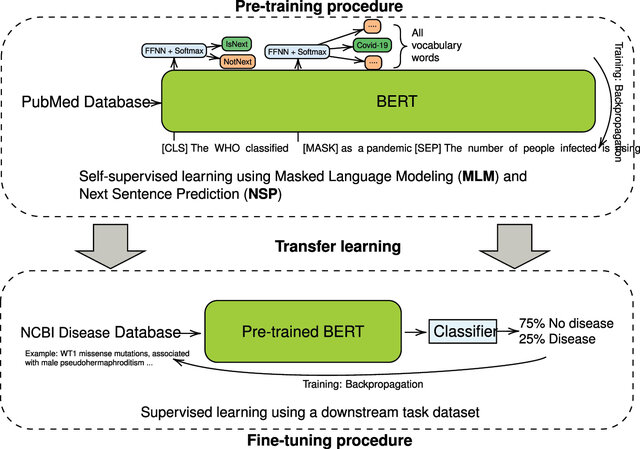
\includegraphics[width=0.6\textwidth]{../assets/figures/ch09-board-emb-img04.png}}
  \caption{فرایند پیش‌آموزش و انتقال یادگیری برای \eng{BERT}: بالا، پیش‌آموزش خودنظارتی با \eng{MLM} و \eng{NSP} (دو سر خروجی روی مدل)؛ پایین، قرار دادن یک دسته‌بند روی \eng{BERT} پیش‌آموزش‌دیده و آموزش تکمیلی با داده برچسب‌دار \eng{Task} هدف. \textit{(برگرفته از تختهٔ کلاس)}}
  \label{fig:ch09-bert}
\end{figure}

\eng{BERT} یک \eng{Transformer Encoder} دوطرفه است. \eng{BERT-Base}: ۱۲ لایه، بُعد ۷۶۸، حدود ۱۱۰ میلیون پارامتر؛ \eng{BERT-Large}: ۲۴ لایه، بُعد ۱۰۲۴. برای ورودی با ۷۱ توکن، خروجی هر لایه $H\in\mathbb{R}^{71\times768}$ است (یک بردار برای هر توکن). سر \eng{MLM} روی لایهٔ ۱۲ قرار می‌گیرد: بردار $1\times768$ موقعیت ماسک با لایهٔ $768\times768$ و سپس $768\times V$ به لاجیت‌هایی به‌طول $V=30522$ می‌رسد و \eng{Softmax} احتمال هر واژهٔ فرهنگ را می‌دهد.

\begin{correctionbox}{جزئیات دقیق \eng{BERT} و وضعیت \eng{NSP}}
در \eng{MLM} حدود ۱۵ درصد توکن‌ها انتخاب می‌شوند (۸۰ درصد با \lr{[MASK]}، ۱۰ درصد توکن تصادفی، ۱۰ درصد بدون تغییر). پژوهش‌هایی مانند \eng{RoBERTa} نشان دادند حذف \eng{NSP} آسیبی نمی‌زند؛ پس \eng{NSP} ضروری نیست. عدد $30522$ اندازهٔ واژگان \eng{bert-base-uncased} است و $V$ به مدل بستگی دارد.
\end{correctionbox}

پس از پیش‌آموزش، سر \eng{MLM} حذف و وزن‌های لایه‌ها نگه داشته می‌شود. دو شیوهٔ استفاده:
\begin{enumerate}
  \item \textbf{استخراج بردار}: جمله را به شبکه می‌دهیم؛ خروجی لایهٔ ۱۲ برای هر واژه یک بردار ۷۶۸‌تایی است (\eng{Embedding} بافتی آن واژه)، و میانگین روی واژه‌ها یک \eng{Embedding} برای کل جمله می‌دهد.
  \item \textbf{انتقال یادگیری} (\eng{Transfer Learning}): روی شبکه یک دسته‌بند می‌گذاریم و با داده‌ای محدود و مرتبط با \eng{Task} خود آموزش تکمیلی (\eng{Fine-tuning}) می‌دهیم.
\end{enumerate}

\begin{exambox}{آیا افزودن لایهٔ بیشتر (\eng{Linear} یا \eng{MLP}) همیشه بهتر است؟}
نمی‌توان قطعی گفت؛ اگر یک لایهٔ ساده کافی است، پیچیده‌ترکردن لازم نیست، و تصمیم بر اساس خطای آموزش و اعتبارسنجی و بایاس/واریانس گرفته می‌شود.
\end{exambox}

\section{قیاس برداری (\eng{Analogy}) در فضای \eng{Embedding}}

اگر روابط معنایی یا ساختاری در فضای \eng{Embedding} خوب بازتاب یافته باشند، اختلاف بردارهای دو جفت واژهٔ هم‌رابطه تقریباً یکسان است:
\[
\vec{v}_{\text{\lr{king}}}-\vec{v}_{\text{\lr{man}}}+\vec{v}_{\text{\lr{woman}}}\approx\vec{v}_{\text{\lr{queen}}}
\quad\Longleftrightarrow\quad
\vec{v}_{\text{\lr{woman}}}-\vec{v}_{\text{\lr{man}}}\approx\vec{v}_{\text{\lr{queen}}}-\vec{v}_{\text{\lr{king}}} .
\]
یعنی «جهت» مفهوم زن‌بودن در برابر مرد‌بودن در دو جفت یکی است. استاد توضیح داد چنین الگوهایی نشانهٔ سازمان‌یافتگی مفید فضا هستند اما برای همهٔ واژه‌ها و مدل‌ها تضمین‌شده نیستند.

همین ایده در گفتار هم مطرح است: مقالهٔ «\lr{[b] = [d] − [t] + [p]}» (چوی و همکاران) گزارش می‌کند که در بازنمایی مدل‌های گفتاری خودنظارتی، جهت‌های خطی متناظر با ویژگی‌های واجی وجود دارد؛ تفاضل $[d]-[t]$ یک «بردار واک‌داری» (\eng{Voicing}) است و افزودن آن به $[p]$ تقریباً $[b]$ می‌دهد. روی تخته:
\[
\vec{v}_{[d]}-\vec{v}_{[t]}+\vec{v}_{[p]}\approx\vec{v}_{[b]},\qquad\text{یعنی}\qquad \vec{v}_{[d]}-\vec{v}_{[t]}\approx\vec{v}_{[b]}-\vec{v}_{[p]}.
\]
کاربردهای مطرح‌شده در کلاس: کشف ویژگی‌های آموخته‌شدهٔ مدل، بررسی لهجه و کاربرد احتمالی در سنتز و \eng{Voice Cloning} (ایده‌ای قابل بررسی، نه نتیجهٔ قطعی).

\begin{correctionbox}{محدودیت‌های قیاس برداری}
قیاس‌هایی مانند king - man + woman در مثال‌های خوب‌انتخاب‌شده و \eng{Embedding} ایستا دیده می‌شوند اما همیشه برقرار نیستند و می‌توانند سوگیری داده را منعکس کنند؛ ابزاری شهودی است، نه قانون.
\end{correctionbox}

\section{کاوش (\eng{Probing}) و تفسیرپذیری}
\label{sec:ch09-probing}

درون جعبهٔ سیاه شبکه هر لایه چه اطلاعاتی نگه می‌دارد؟ استاد \eng{Probing} را به پروب‌زدن در نقاط مختلف یک مدار الکترونیکی تشبیه کرد.

\begin{definitionbox}{\term{دسته‌بند کاوشگر}{Probing Classifier}}
\eng{Probe} یک مدل کوچک و ساده (معمولاً خطی) است که روی خروجی یک لایهٔ مشخص از یک شبکهٔ آموزش‌دیده و \emph{منجمد‌شده} آموزش داده می‌شود تا یک ویژگی زبانی یا گفتاری را پیش‌بینی کند. دقت آن نشان می‌دهد آن اطلاعات در آن لایه تا چه حد «قابل استخراج» است.
\end{definitionbox}

مراحل: (۱) مدل پیش‌آموزش‌دیده را فریز کن؛ (۲) یک لایه (مثلاً میانی) انتخاب کن؛ (۳) نمایش‌های آن را برای داده‌ای برچسب‌دار (مثلاً \eng{Manner of Articulation} هر توکن) استخراج کن؛ (۴) یک دسته‌بند کوچک آموزش بده؛ (۵) دقت را روی داده‌ای کنار گذاشته‌شده بسنج. هدف اصلی از نگاه استاد این نیست که ویژگی دقیقاً در کدام لایه آموخته شده، بلکه این است که آیا مدل اساساً آن را یاد گرفته (مثلاً اطلاعات واجی، زبان، گوینده، تفکیک واکه و خیشومی).



برای تجسم \eng{Embedding}ها از کاهش بُعد (\eng{PCA}، \eng{t-SNE}) استفاده می‌شود، ولی استاد تأکید کرد که دیدن دو کلاس جدا در تصویر به‌تنهایی ثابت نمی‌کند مدل آن اطلاعات را خوب یاد گرفته؛ باید یک \eng{Task} تعریف و عملکرد را کمّی سنجید.

این مباحث در چارچوب \term{هوش مصنوعی توضیح‌پذیر}{Explainable AI} و \term{تفسیرپذیری}{Interpretability} قرار می‌گیرند. (\eng{Visualization}: نمایش هندسی و عمدتاً بصری برای درک شهودی؛ \eng{Probing}: معیار کمّی مبتنی بر یک \eng{Task}.)

\begin{correctionbox}{\eng{Probing} چه چیزی را ثابت می‌کند؟}
دقت بالای پروب نشان می‌دهد اطلاعات \emph{وجود دارد و قابل استخراج است}، نه اینکه مدل از آن برای \eng{Task} اصلی \emph{استفاده می‌کند}. پروب را ساده (خطی) می‌گیرند تا خودش \eng{Task} را یاد نگیرد، و دقت را با یک مبنا (مثلاً مدل با وزن‌های تصادفی) مقایسه می‌کنند.
\end{correctionbox}

\section{بازگشت به \eng{TTS}: تلفظ درست هر واژه}

پس از \term{نرمال‌سازی متن}{Text Normalization}، \eng{Front-End} باید تلفظ را با \term{تبدیل نویسه به واج}{Grapheme-to-Phoneme, G2P} مشخص کند. چون در فارسی بسیاری از حرکات کوتاه نوشته نمی‌شوند، دو دشواری داریم: \term{هم‌نویسه‌ها}{Homograph} (یک نوشتار با تلفظ‌های متفاوت) و \term{واژه‌های خارج از واژگان}{Out-of-Vocabulary, OOV} (واژه‌ای که در فرهنگ تلفظ نیست).

\begin{table}[htbp]
\centering
\small
\begin{tabular}{p{2.0cm}p{4.2cm}p{4.2cm}p{3.2cm}}
\toprule
\textbf{نوشتار} & \textbf{تلفظ و معنی ۱} & \textbf{تلفظ و معنی ۲} & \textbf{ابزار تفکیک}\\
\midrule
مرد & \lr{/mæɾd/} «انسان مذکر» (اسم) & \lr{/moɾd/} «درگذشت» (فعل) & نقش دستوری (\eng{POS})\\
کرم & \lr{/keɾm/} «جانور خاکی»؛ \lr{/keɾem/} «ماده مرطوب‌کننده» & \lr{/kæɾæm/} «بخشندگی» (مثال افزوده) & معنای بافتی\\
گرم & \lr{/gæɾm/} «داغ» & \lr{/geɾæm/} «واحد جرم» & معنای بافتی\\
\bottomrule
\end{tabular}
\caption{نمونه‌هایی از هم‌نویسه‌های فارسی (نمادهای \eng{IPA} تقریبی‌اند).}
\end{table}

بسیاری از هم‌نویسه‌ها با نقش دستوری قابل تفکیک‌اند («او مُرد» فعل، «آن مَرد رفت» اسم؛ یک برچسب‌زن \eng{POS} مثل \eng{hazm} کافی است). اما برای دو واژهٔ هم‌نقش، مثل «کِرم» خاکی و «کِرِم» مرطوب‌کننده که هر دو اسم‌اند، برچسب دستوری کمکی نمی‌کند و به \eng{Embedding} بافتی نیاز داریم.

\subsection{طرح مهندسی: از ارزان به گران}
مسیر پیشنهادی استاد (شکل~\ref{fig:ch09-flow}): اگر واژه در فرهنگ هست و یک تلفظ دارد، جست‌وجوی مستقیم؛ اگر چند تلفظ دارد، دسته‌بند بافتی؛ اگر نیست (\eng{OOV})، شکستن به نویسه‌ها و مدل \eng{G2P} از نوع \eng{Sequence-to-Sequence}.

\begin{figure}[htbp]
\centering
\begin{tikzpicture}[rtl, 
  node distance=0.7cm and 0.5cm,
  box/.style={draw,rounded corners=2pt,minimum height=0.8cm,align=center,fill=blue!6,font=\small,inner sep=4pt},
  dec/.style={draw,diamond,aspect=2.2,align=center,fill=yellow!15,font=\small,inner sep=1pt},
  ar/.style={-{Stealth[length=2mm]},thick}]
  \node[box] (w) {واژه پس از نرمال‌سازی متن};
  \node[dec,below=0.6cm of w] (d1) {در فرهنگ\\هست؟};
  \node[dec,below left=1cm and 0.5cm of d1] (d2) {چند تلفظ\\دارد؟};
  \node[box,below right=1.1cm and 0.8cm of d1] (g2p) {مدل \lr{G2P}\\\lr{Seq2Seq}};
  \node[box,below left=1cm and 0.1cm of d2] (cls) {دسته‌بند بافتی\\\lr{Global Classifier}};
  \node[box,below right=1cm and 0.1cm of d2] (lk) {جست‌وجوی مستقیم\\در فرهنگ};
  \draw[ar] (w)--(d1);
  \draw[ar] (d1)-|node[pos=0.25,above,font=\scriptsize]{بله}(d2);
  \draw[ar] (d1)-|node[pos=0.25,above,font=\scriptsize]{خیر: \lr{OOV}}(g2p);
  \draw[ar] (d2)-|node[pos=0.25,above,font=\scriptsize]{بله}(cls);
  \draw[ar] (d2)-|node[pos=0.25,above,font=\scriptsize]{خیر}(lk);
\end{tikzpicture}
\caption{طرح تصمیم برای یافتن تلفظ: تا جای ممکن از روش‌های ارزان‌تر استفاده می‌شود. (شکل افزوده)}
\label{fig:ch09-flow}
\end{figure}

\subsection{رفع ابهام هم‌نویسه با دسته‌بندی}
انتخاب یکی از چند تلفظ متناسب با جمله یک مسئلهٔ دسته‌بندی (و برای بیش از دو تلفظ، چندکلاسه) است. ورودی دسته‌بند \eng{Embedding} بافتی واژه است: جمله را به مدلی مثل \eng{BERT} می‌دهیم و بردار موقعیت واژهٔ مبهم را به دسته‌بند می‌دهیم.

\textbf{چرا یک دسته‌بند سراسری} (\term{دسته‌بند سراسری}{Global Classifier}) و نه یکی برای هر هم‌نویسه (مثلاً ۵۰۰ مدل)؟ پرسش کلاسی با دو پاسخ استاد:
\begin{enumerate}
  \item \textbf{اشتراک ویژگی‌ها}: نشانه‌های لازم (قواعد نحوی، ساختاری، معنایی؛ مثلاً «اگر قبل از کلمه حرف تعریف، ضمیر ملکی یا صفت آمد، کلمه اسم است») میان واژه‌ها مشترک است و یک مدل مشترک آن‌ها را یک بار یاد می‌گیرد.
  \item \textbf{کمبود داده}: برخی هم‌نویسه‌ها نمونهٔ کم دارند و مدل جداگانه روی آن‌ها بیش‌برازش می‌شود یا یاد نمی‌گیرد؛ با وزن‌های مشترک، دانش از واژه‌های پرتکرار به کم‌تکرار منتقل می‌شود (\eng{Cross-word Transfer Learning}).
\end{enumerate}

\textbf{ماسک‌کردن کلاس‌های نامعتبر:} برای اینکه فقط تلفظ‌های معتبر همان واژه انتخاب شوند، پیش از \eng{Softmax} لاجیت تلفظ‌های نامعتبر را $-\infty$ می‌گذاریم:
\[
z_i'=\begin{cases} z_i & \text{اگر تلفظ } i \text{ برای این واژه معتبر باشد},\\ -\infty & \text{در غیر این صورت,}\end{cases}
\qquad P_i=\operatorname{Softmax}(z')_i .
\]
روی تخته برای «گرم»: «گرفتن بیشینه فقط روی واج‌های مرتبط». در استنتاج هم \eng{Greedy}/\eng{Argmax} به‌کار می‌رود، چون هدف تلفظ درست است و به تنوع نیاز نداریم.

\begin{addedbox}{مثال عددی: ماسک‌کردن}
برای «گرم» لاجیت‌ها: \eng{garm}:~$2.0$، \eng{geram}:~$0.5$ و تلفظ نامعتبر دیگر: $3.0$. بدون ماسک احتمال‌ها $(0.254,\,0.057,\,0.690)$ است و کلاس نامعتبر برنده می‌شود؛ با ماسک فقط دو کلاس معتبر می‌مانند، $(0.818,\,0.182)$، و \eng{garm} انتخاب می‌شود.
\end{addedbox}

\section{واژه‌های ناشناخته و \eng{G2P} از نوع \eng{Sequence-to-Sequence}}

برای واژهٔ \eng{OOV} جست‌وجوی مستقیم ممکن نیست؛ واژه را به نویسه‌ها می‌شکنیم و مدل با تکیه بر الگوهای دادهٔ آموزشی تلفظ را پیش‌بینی می‌کند. داده را از خود فرهنگ تلفظ می‌سازیم: ورودی دنبالهٔ نویسه‌ها و خروجی دنبالهٔ واج‌ها،
\[
[g_1,g_2,\dots,g_n]\;\longrightarrow\;[p_1,p_2,\dots,p_m],\qquad n\neq m \text{ (در حالت کلی)}.
\]
نمونه: «مدرسه» ۵ نویسه (م، د، ر، س، ه) ولی ۷ واج (\lr{m æ d ɾ e s e}) دارد، چون حرکات کوتاه نوشته نمی‌شوند؛ «خواب» ۴ نویسه و ۳ واج (\lr{x ɒ b}) دارد چون «و» تلفظ نمی‌شود. پس نمی‌توان برای هر نویسه یک واج فرض کرد.

\subsection{چرا \eng{Seq2Seq} و معماری رمزگذار–رمزگشا؟}
دسته‌بندی چندکلاسه یک ورودی را به یکی از کلاس‌های ثابت می‌نگارد، اما در \eng{G2P} باید \emph{دنباله‌ای} با طول وابسته به ورودی و از پیش نامعلوم تولید کنیم؛ این مسئلهٔ \term{دنباله به دنباله}{Sequence-to-Sequence} است.
\begin{itemize}
  \item \textbf{رمزگذار} (\eng{Encoder}): دنبالهٔ نویسه‌ها را به نمایشی تبدیل می‌کند که اطلاعات لازم برای تولید تلفظ را دارد. به رمزگشا یا یک \eng{Context Vector} (خلاصهٔ ورودی) می‌دهد یا، با \eng{Attention}، همهٔ حالت‌های خروجی رمزگذار را در دسترس می‌گذارد.
  \item \textbf{رمزگشا} (\eng{Decoder}): واج‌ها را گام‌به‌گام تولید می‌کند، با استفاده از ورودی رمزگذاری‌شده، واج‌های قبلی و حالت فعلی خودش.
\end{itemize}

\begin{figure}[htbp]
\centering
\begin{tikzpicture}[rtl, 
  tok/.style={draw,minimum width=0.85cm,minimum height=0.7cm,font=\small,fill=green!10},
  ph/.style={draw,minimum width=0.85cm,minimum height=0.7cm,font=\small,fill=orange!15},
  enc/.style={draw,rounded corners=3pt,minimum width=5.2cm,minimum height=0.9cm,fill=blue!10,font=\small},
  ar/.style={-{Stealth[length=2mm]},thick}]
  % graphemes (RTL reading kept as written order left-to-right for the toy figure)
  \foreach \i/\c in {1/م,2/د,3/ر,4/س,5/ه}{\node[tok] (g\i) at ({(6-\i)*0.95},0) {\c};}
  \node[enc] (E) at (2.85,1.5) {رمزگذار: \lr{Encoder}};
  \foreach \i in {1,...,5}{\draw[ar] (g\i)--(g\i |- E.south);}
  \node[enc,fill=orange!15,minimum width=5.8cm] (D) at (2.85,3.4) {رمزگشا: \lr{Decoder} + \lr{Cross-Attention}};
  \draw[ar] (E)--(D) node[midway,right,font=\scriptsize]{نمایش‌های ورودی};
  \foreach \i/\c in {1/m,2/æ,3/d,4/ɾ,5/e,6/s,7/e}{\node[ph] (p\i) at (\i*0.78-0.4,4.9) {\lr{\c}};}
  \foreach \i in {1,...,7}{\draw[ar] (D.north -| p\i)--(p\i);}
  \node[anchor=east,font=\small] at (0.3,0) {نویسه‌ها:};
  \node[anchor=east,font=\small] at (-0.05,4.9) {واج‌ها:};
\end{tikzpicture}
\caption{مدل \eng{G2P} با رمزگذار–رمزگشا برای واژهٔ «مدرسه» (۵ نویسه به ۷ واج). (شکل افزوده)}
\end{figure}

\textbf{\eng{Cross-Attention}.} در \eng{Self-Attention} یک دنباله به عناصر خودش توجه می‌کند؛ در \eng{Cross-Attention} رمزگشا به نمایش‌های دنبالهٔ دیگر (خروجی رمزگذار) توجه می‌کند: \eng{Query} از رمزگشا و \eng{Key} و \eng{Value} از رمزگذار می‌آیند. پس هنگام تولید واج بعدی، رمزگشا به بخش‌های مرتبط ورودی نگاه می‌کند. (در \eng{Embedding} بافتی هدف نمایش یک عنصر با توجه به متن خودش بود؛ در رمزگذار–رمزگشا رمزگشا به دنبالهٔ ورودی مراجعه می‌کند.)

مسائل دیگر از نوع \eng{Seq2Seq}: \term{ترجمهٔ ماشینی}{Machine Translation} و \term{خلاصه‌سازی انتزاعی}{Abstractive Summarization}. برای \eng{OOV} مدل بایت‌محور \eng{ByT5} هم روی تخته ذکر شد.

\section{ملاحظات مهندسی \eng{G2P} و بحث پایانی}

پرسش دانشجو: چرا همه‌چیز را با \eng{Seq2Seq} حل نکنیم؟ پاسخ استاد: یک تصمیم مهندسی است و روش‌ها از نظر هزینه، داده و پیچیدگی فرق دارند. ترتیب پیشنهادی: (۱) فرهنگ برای واژه‌های با تلفظ مشخص (بسیار کم‌هزینه)؛ (۲) دسته‌بند برای هم‌نویسه‌ها؛ (۳) \eng{G2P} برای \eng{OOV}. باید از راه‌حل ارزان‌تر شروع کرد («اصفهانی‌بودن در مهندسی»).

\begin{exambox}{آیا همیشه باید از فرهنگ شروع کنیم؟}
خیر؛ قاعدهٔ مهندسی است، نه الزام. اگر فرهنگ مناسبی نیست یا متن پر از واژه‌های جدید و محاوره‌ای است، استفادهٔ مستقیم از \eng{G2P} منطقی است.
\end{exambox}

\begin{correctionbox}{ذخیرهٔ خروجی \eng{OOV}}
نتیجهٔ \eng{G2P} را می‌توان ذخیره (\eng{Cache}) کرد تا هزینهٔ استنتاج کم شود، ولی اگر تلفظ به بافت وابسته باشد ذخیرهٔ تلفظ ثابت مناسب نیست. ذخیره به‌معنای آموزش مجدد یا به‌روزرسانی وزن‌ها نیست و تلفظ خودکار پیش از افزودن دائمی به فرهنگ باید بازبینی شود (پیشنهاد افزوده).
\end{correctionbox}

\section{جمع‌بندی}

لایهٔ خروجی و خطا را بر اساس نوع مسئله انتخاب می‌کنیم؛ آموزش (با حقیقت مبنا) با استنتاج (\eng{Greedy}، \eng{Top-k}، \eng{Top-p}، \eng{Temperature}) فرق دارد. \eng{Embedding} ایستا یک جدول جست‌وجوست و بافتی تابعی از کل جمله (\eng{Self-Attention} یا \eng{LSTM}؛ پیش‌آموزش خودنظارتی \eng{BERT}). در \eng{TTS}: فرهنگ برای واژه‌های معمول، دسته‌بند سراسری با ماسک برای هم‌نویسه‌ها، و \eng{G2P} رمزگذار–رمزگشا برای واژه‌های ناشناخته.

\begin{exambox}{نکات مهم برای مرور و امتحان}
\begin{enumerate}
  \item معماری و لایهٔ خروجی را بر اساس \eng{Task} طراحی کنید و بدون توجه به عملکرد لایه نیفزایید؛ خطای آموزش کافی نیست، خطای اعتبارسنجی و بایاس/واریانس را هم ببینید.
  \item ایستا = جدول جست‌وجو (فایل بردارها)؛ بافتی = وزن‌های شبکه، بردار فقط پس از دادن جمله. \eng{Contextual Embedding} را با \eng{Transformer} یکی نگیرید (\eng{Attention}، \eng{LSTM}).
  \item به \eng{Visualization} اکتفا نکنید؛ \eng{Probing} شواهد کمّی می‌دهد.
  \item در \eng{TTS}، هم‌نویسه‌ها و \eng{OOV} دو چالش متفاوت‌اند و با روش‌های متفاوت حل می‌شوند.
  \item دلایل دسته‌بند سراسری برای هم‌نویسه‌ها: اشتراک ویژگی‌ها و کمبود داده؛ در استنتاج کلاس‌های نامعتبر ماسک می‌شوند و \eng{Argmax} به کار می‌رود.
  \item \eng{G2P} برای \eng{OOV} از نوع \eng{Seq2Seq} است چون طول دنبالهٔ واج‌ها لزوماً برابر طول دنبالهٔ نویسه‌ها نیست.
  \item تا جای ممکن از فرهنگ و روش‌های ساده‌تر (ارزان‌تر) شروع کنید و مدل‌های پیچیده را فقط در صورت نیاز وارد کنید.
\end{enumerate}
\end{exambox}
